\documentclass[               %
  unicode,                    % 文字コードの指定
  mathserif,                  %
  m,                          % vertical position of text: (t,m,b)
  % handout,                  % for printing slides
  aspectratio=169,            % 画面サイズを(16:9)にする
  12pt,                       % フォント基本サイズを12ptにします
  % compress,
  unknownkeysallowed
]{beamer}
%
% 各種設定用ファイルの読み込み:ここのファイル名は決め打ちにさせてください
%
  %
% パッケージの選択
%
\usepackage{luatexja}% 日本語に
\usepackage[haranoaji,deluxe]{luatexja-preset}% フォント指定
\renewcommand{\kanjifamilydefault}{\gtdefault}% 既定をゴシック体に
\usepackage{url}              % LaTeXの文章内にURLを貼りたいとき
\usepackage{hyperref}         % TeX 文書(DVI、PDF など)に HTML と同じハイパーリンク 機能を加えるためのマクロ
\usepackage{siunitx}          % LATEX で SI単位(国際単位系)を出力する
\usepackage{enumitem}         % リスト環境のレイアウトを制御
\usepackage{tikz}             % TeX 用の描画パッケージ
\usepackage{
    amsmath, % 環境
    amssymb, % 記号
    amsfonts % 特殊文字
}                             % amsmathの数式環境
\usetikzlibrary{positioning}     % ”positioning”ライブラリ
\usetikzlibrary{shapes.callouts} % 吹き出しの形を使うためにshapesライブラリを利用します
\usepackage[absolute,overlay]{textpos} % textposパッケージ
%\usepackage[colorgrid,gridunit=pt,texcoord]{eso-pic}
             % eso-picパッケージを使ってスライドの上からグリッドを表示、リリース時は消しておく
%\usepackage{layout}
             % layout パッケージもリリース時は消す
%
% デザインの選択
%     ここではテーマとしてmetropolisを読込
%
\usetheme[
    block=fill, % ブロックに背景をつける
    numbering=fraction % 合計ページ数を表示
]{metropolis}

%
% ここからはページの見え方の設定
%
% ページ番号
\setbeamerfont{frame numbering}{size=\large}
%
% CUD 配色の作成
% cf. http://bit.ly/2G99WCG
\definecolor{cud_blue}{rgb}{.109803922,.349019608,.682352941}
\definecolor{cud_green}{rgb}{.282352941,.639215686,.407843137}
\definecolor{cud_orange}{rgb}{.929411765,.564705882,.156862745}
\definecolor{cud_lightgray}{rgb}{.784313725,.784313725,.796078431}
%
% 基本色の変更
\setbeamercolor{normal text}{fg=cud_blue}
\setbeamercolor{example text}{fg=cud_green}
\setbeamercolor{alerted text}{fg=cud_orange}
%
% Navigation symbol は不要なので消す
\setbeamertemplate{navigation symbols}{}
%
% 見出しのスペースを消したい
\setbeamertemplate{frametitle}{
  \nointerlineskip
  \begin{beamercolorbox}[wd=\paperwidth,ht=2.25ex,dp=0.75ex]{frametitle} % htで直接指定
    \hspace*{1ex}\insertframetitle % 左margin + hspaceから始める
  \end{beamercolorbox}
}
%
% 図表番号を「図1」「表1」とかにする
\renewcommand{\figurename}{図}
\renewcommand{\tablename}{表}
\setbeamertemplate{caption}[numbered]
%
% 図とキャプションの間の余白
\setlength\abovecaptionskip{0pt}
%
% highlight マクロ tasusu.github.io/tikz.html から頂きました
\newcommand{\highlight}[2][yellow]{\tikz[baseline=(x.base)]{\node[rectangle,rounded corners,fill=#1!10](x){#2};}}
\newcommand{\highlightcap}[3][yellow]{\tikz[baseline=(x.base)]{\node[rectangle,rounded corners,fill=#1!10](x){#2} node[below of=x, color=#1]{#3};}}
%
%footer修正
\def\logoC{opencae-logo.png}
\def\logoD{kotohajime.png}
\makeatletter
\setbeamertemplate{footline}{
    \begin{columns}[totalwidth=160mm]
      \begin{column}{24.1mm}
        \includegraphics[width=24.1mm, height=5mm]{work/images/\logoC}
      \end{column}
      \begin{column}{104mm}
         {\scriptsize \color{cud_lightgray} \insertshortinstitute / \insertshortdate{}  (\insertshortauthor) }
      \end{column}
      \begin{column}{16mm}
         {\footnotesize \color{cud_orange} \rightline{ \insertframenumber{} / \inserttotalframenumber}}
      \end{column}
      \begin{column}{15mm}
        \includegraphics[width=15mm, height=5mm]{work/images/\logoD}
      \end{column}
    \end{columns}
}
   % 資料毎に変えない設定を読み込む
  % 表題の例
%     title     に主題
%     subtittle に副題を設定(省略可)
%
\title{圧力容器の応力値を手計算とCAEで比較した}
\subtitle{~ PrePoMaxは、やればできる子~}
%
% 日付/発表者設定の例
%     date      に発表日の日付
%     author    に発表者の名前
%     institute には本来は発表者の所属先ですが、下の例では発表会の名前とした
%     それぞれ左の角カッコ内が簡易表記で、表紙以外で使われ
%     右の波カッコ内が詳細表記で、表紙で使われる
%
\date[2-24-2024]{発表日:2024年2月24日}
\author[ichmy55]{発表者:ichmy55}
\institute[  25th Meeting/OpenCAE Local User Group@Kantou(str)]{報告:第25回オープンCAE勉強会@関東(構造など)}
  % 資料毎に変える設定を読み込む
%
% ここから、各章毎に分割したソースファイルを順番に読込
%
\begin{document}
  %
  \maketitle                         % 表紙
  \begin{frame}{はじめに}
  \begin{itemize}[itemsep=2.5ex, leftmargin=3mm]
      \large
      \item[〇] 報告者がCAEを始めたて初心者の時点で(商用コードで)出来て

                いたことを、OpenCAEで再現した

      \item[〇] 上記のうち、メッシュ切について日本語で説明している資料が少ないのが残念

      \item[〇] 最近OpenCAEでも簡単に切れるようになった6面体

                メッシュを 中心に、まとめてみた
  \end{itemize}
\end{frame}
          % はじめに
  \begin{frame}{本日の流れ}
  \begin{itemize}
     \item[▶] \highlight[cud_yellow]{目次}
     \begin{itemize}[itemsep=1.3ex, leftmargin=1cm]
       \item[1.] 自己紹介
       \item[2.] OpenCAEの構造解析でもメッシュにこだわりたい
       \item[3.] 本日の例題と以前の勉強会で報告された結果
       \item[4.] 改めて解いてみた(PrePoMaxは、やればできる子)
       \item[5.] まとめ
       \item[A.] 付録 ~ソースのありか~
    \end{itemize}
  \end{itemize}
\end{frame}
           % 目次
  %%%
  %%%
  \begin{frame}{本日の流れ}
  \begin{itemize}
     \item[] 目次
     \begin{itemize}[itemsep=1.3ex, leftmargin=1cm]
        \item[▶1.] \highlight[cud_yellow]{ 自己紹介}
        \item[2.] 報告者が当時出来ていたこと
        \item[3.] 本日の例題と以前の勉強会で報告された結果
        \item[4.] あらためて解いてみた
        \item[5.] まとめ
     \end{itemize}
  \end{itemize}
\end{frame}
           % 
  \begin{frame}{自己紹介}
  \begin{table}[hbtp]
      \begin{tabular}{rl} % 表は項目名を右寄せ、データを左寄せ
      ハンドル名 & ichmy55(いちみーごーごー)で活動してます \\
      職業       & 普段は某企業で構造解析をやってます  \rule[0mm]{0mm}{7mm} \\
      CAE歴      & 10年ほど前から某商用ソフトを使ったCAEに従事 \rule[0mm]{0mm}{7mm} \\
                 & その前は単なるソフト屋でした \\
      情報発信   & Github : {\urlstyle{same} \color{cud_orange}
                             \href{https://github.com/ichmy55/opencae-slides}{@ichmy55}}
                   (本スライドのソースを置いています) \rule[0mm]{0mm}{7mm}\\
                 & Docswell : {\urlstyle{same} \color{cud_orange}
                             \href{https://www.docswell.com/user/ichmy55}{@ichmy55}}
                   (同PDFファイルを置いています) \\
                 & \\
    \end{tabular}
  \end{table}
\end{frame}
    % 自己紹介
  %%%
  \begin{frame}{本日の流れ}
  \begin{itemize}
      \item[] 目次
      \begin{itemize}[itemsep=1.3ex, leftmargin=1cm]
        \item[1.]  {\color{cud_lightgray} 自己紹介}
        \item[▶2.] \highlight[cud_yellow]{ 報告者が当時出来ていたこと }
        \item[3.] 本日の例題と以前の勉強会で報告された結果
        \item[4.] 改めて解いてみた(PrePoMaxは、やればできる子)
        \item[5.] まとめ
     \end{itemize}
  \end{itemize}
\end{frame}
           % 
  \begin{frame}{報告者が当時出来ていたこと}
  \begin{table}[hbtp]
      \caption{報告者が当時出来ていたこと}
      \begin{tabular}{|r|l|} % 表は項目名を右寄せ、データを左寄せ
          \hline
          形状     & 3次元形状のみ \rule[0mm]{0mm}{7mm} \\
          \hline
          材質     & 線形弾性体のみ \rule[0mm]{0mm}{7mm} \\
          \hline
          メッシュ & 主に4面体、一部 \highlight[cud_lightpink]{6面体}\rule[0mm]{0mm}{7mm} \\
                   &  \\
          \hline
          境界条件 & 変位拘束と荷重(分布or集中) \rule[0mm]{0mm}{7mm} \\
          \hline
          結果処理 & 反力のチェックサム \rule[0mm]{0mm}{7mm} \\
                   & 接点データ外だし→表計算ソフトでグラフ化 \\
          \hline
          \multicolumn{2}{c}{これらをOpenCAEで試してみる}  \rule[0mm]{0mm}{7mm}
    \end{tabular}
  \end{table}
\end{frame}
      % 
  %%%
  \begin{frame}{本日の流れ}
  \begin{itemize}
      \item[] 目次
      \begin{itemize}[itemsep=1.3ex, leftmargin=1cm]
        \item[1.] {\color{cud_lightgray} 自己紹介}
        \item[2.] {\color{cud_lightgray} 報告者が当時出来ていたこと}
        \item[▶3.] \highlight[cud_yellow]{ 本日の例題と以前の勉強会で報告された結果}
        \item[4.] 改めて解いてみた
        \item[5.] まとめ
     \end{itemize}
  \end{itemize}
\end{frame}
           % 
  \begin{frame}{本日の例題}
 
    \begin{columns}[t]
    \begin{column}{0.65\textwidth}
        \\
        <参考文献\cite{wanted} より例題を拝借> \\
        右\figurename \ref{fig:example-probrem}に示すような圧力容器に内圧10MPaが \\
        かかっている。
        材料はSB450で、ヤング率は205GPa、降伏応力は250MPaである。 \\
        本構造は薄肉構造と近似できるとする。
      \begin{itemize}
          \item{円筒部のA点と半球部のB点の応力状態を求めよ}
          \item{A点とB点ミーゼス相当応力を求め、幸福応力に達する臨界圧力を求めよ}
      \end{itemize}
    \end{column}
    \begin{column}{0.35\textwidth}
      \begin{figure}[htbp]
        \begin{center}
          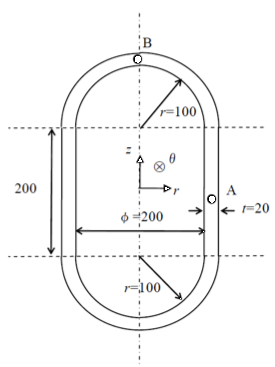
\includegraphics[keepaspectratio,scale=2.2]{work/images/example-probrem.png}
            \caption{本日の例題(圧力容器)} \label{fig:example-probrem}
        \end{center}
      \end{figure}
    \end{column}
  \end{columns}

% 図の挿入
%\begin{figure}[htbp]
%\begin{center}
%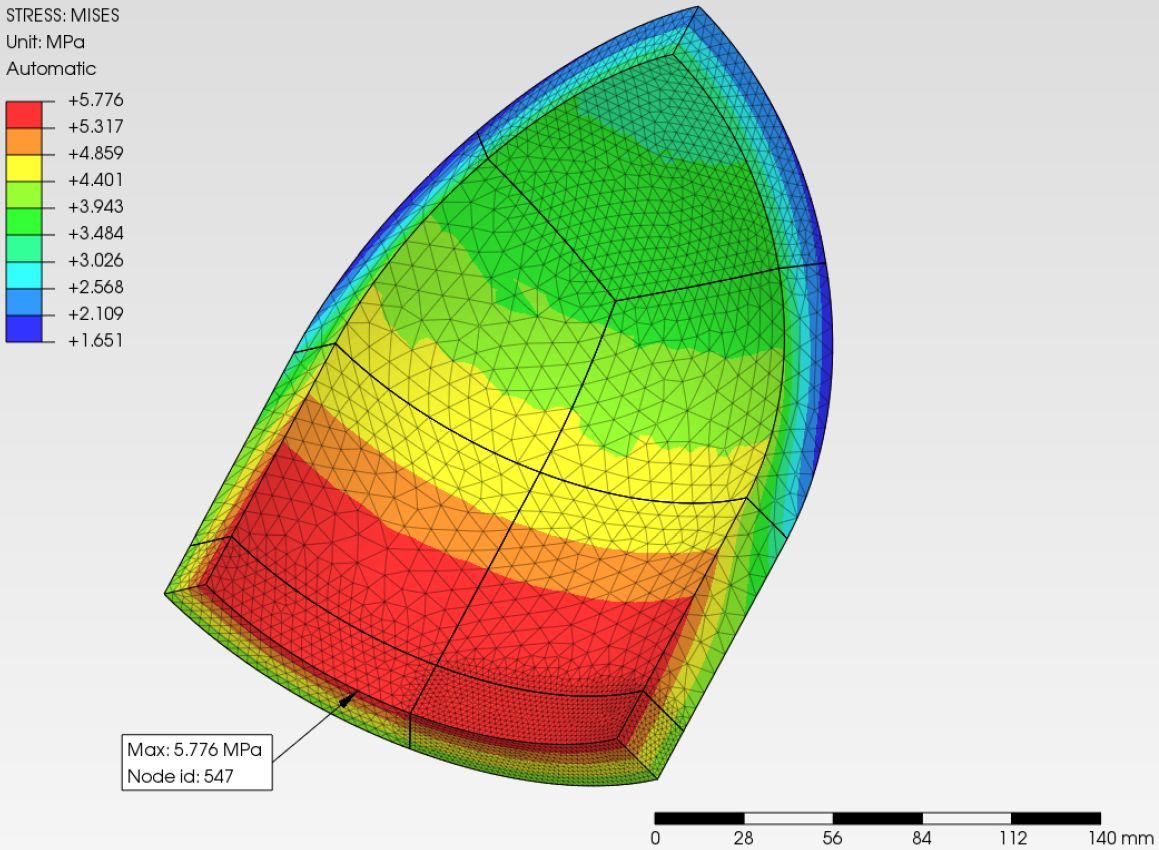
\includegraphics[keepaspectratio,scale=1.0]{work/images/fig01.jpg}
%\caption{4面体メッシュ切り(成功例)}
%\end{center}
%\end{figure}
 
\end{frame}
   % 本日の例題と以前の勉強会で報告された結果
  \begin{frame}{以前の勉強会で報告された結果}
 
    \begin{columns}[t]
    \begin{column}{0.7\textwidth}
       <報告者コメント> \\
         ミーゼス応力で比較した結果、A点応力に差異 \\
          \begin{table}[hbtp]
            \begin{tabular}{rlp{10em}} % 表は項目名を右寄せ、データを左寄せ
               手計算 & 52 MPa & \\
               CAE    & 58.9 MPa  & \\
            \end{tabular}
          \end{table}
        <参加者コメント(一部のみ抜粋し要約)> \\
         \begin{itemize}
            \item[①] コンター図がまだら模様でおかしい。\\
                     \Add{メッシュ}に問題がある。 \\
                     正しく計算したければ \highlight[cud_yellow]{6面体メッシュ}で厚み\\
                     方向に4層切りメッシュを作る必要がある。\\
            \item[②] CAE結果と比較する相手として、薄肉構造を仮定 \\
                     した手計算は相応しくない?
         \end{itemize}
    \end{column}
    \begin{column}{0.3\textwidth}
      \begin{figure}[htbp]
        \begin{center}
          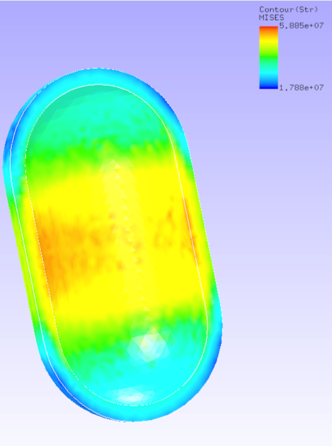
\includegraphics[keepaspectratio,scale=1.5]{work/images/previous.png}
            \caption{以前の勉強会で報告された結果} \label{fig:previous}
        \end{center}
      \end{figure}
    \end{column}
  \end{columns}
  %
  % TiKZを使った図形の描画 図2でA点を指し示す矢印
  \begin{textblock*}{30pt}(385pt,95pt)
    \begin{tikzpicture}
        \draw[->, draw=cud_red, line width=2pt] (0.7,0.8) -- (0,0.3);
        \node[rectangle,fill=cud_yellow,text width=0.5cm,text centered,rounded corners,minimum height=0.5cm](s) at (1cm,1cm) { \scriptsize A点};
    \end{tikzpicture}
  \end{textblock*}
\end{frame}
 % 以前の勉強会でのコメント
  %%%
  \begin{frame}{本日の流れ}
  \begin{itemize}
      \item[] 目次
    \begin{enumerate}[label=\textbf{ \arabic*.},itemsep=1.3ex, leftmargin=1cm]
        \item[1.] 自己紹介
        \item[2.] OpenCAEの構造解析でもメッシュにこだわりたい
        \item[3.] 本日の例題
        \item[▶4.] \highlight[cud_yellow]{ 以前の計算結果と指摘 }
        \item[5.] 改めて解いてみた(PrePoMaxは、やればできる子)
        \item[6.] まとめ
        \item[A.] 付録 ~ソースのありか~
    \end{enumerate}
  \end{itemize}
\end{frame}
           % 改めて解いてみた(PrePoMaxは、やればできる子)
  \begin{frame}{今回の改善点}
 
    \begin{columns}[t]
    \begin{column}{0.7\textwidth}
        <今回の改善点> \\
         \begin{itemize}
            \item[①] コンター図がまだら模様の件 \\
                     これは4面体メッシュでの解析ではやむを得ない \\
                     \Add{6面体メッシュ}を用いてメッシュを切りなおす
            \item[]
            \item[②] 薄肉構造を仮定した件 \\
                     板厚方向に多くの分割数を確保し \\
                     板厚方向の\Add{応力分布}を\Add{厚肉円筒の応力式}と比較
            \item[]
            \item[③] メッシュ数の節約のため、\\
                     1/8ショートケーキモデルとする
         \end{itemize}
    \end{column}
    \begin{column}{0.3\textwidth}
      \begin{figure}[htbp]
        \begin{center}
          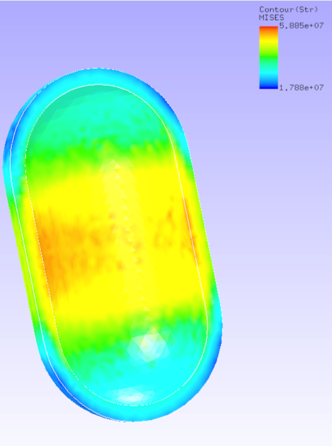
\includegraphics[keepaspectratio,scale=1.5]{work/images/previous.png}
            \caption{以前の勉強会で報告された結果(再掲)}
        \end{center}
      \end{figure}
    \end{column}
  \end{columns}
  %
  % TiKZを使った図形の描画 図2でA点を指し示す矢印
  \begin{textblock*}{30pt}(385pt,95pt)
    \begin{tikzpicture}
        \draw[->, draw=cud_red, line width=2pt] (0.7,0.8) -- (0,0.3);
        \node[rectangle,fill=cud_yellow,text width=0.5cm,text centered,rounded corners,minimum height=0.5cm](s) at (1cm,1cm) { \scriptsize A点};
    \end{tikzpicture}
  \end{textblock*}
\end{frame}
      % 今回の改善点
  \begin{frame}{改めてメッシュ要素について復習}
  \begin{table}[hbtp]
      \caption{3次元構造解析で使われる主なメッシュ要素(一部)<参考文献\cite{handbook}>}
      \vspace{-5mm}
      \begin{tabular}{|r|c|c|c|} % 表は項目名を右寄せ、データを中寄せ
          \hline
          名称       & 4面体2次要素 & 6面体1次要素 & 4面体1次要素 \\
          \hline
          接点配置   & 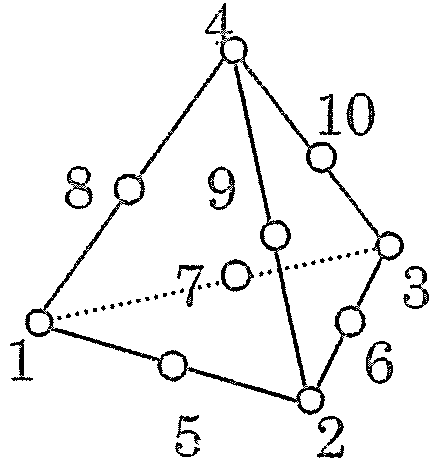
\includegraphics[keepaspectratio]{work/images/tet10.png}
                     & 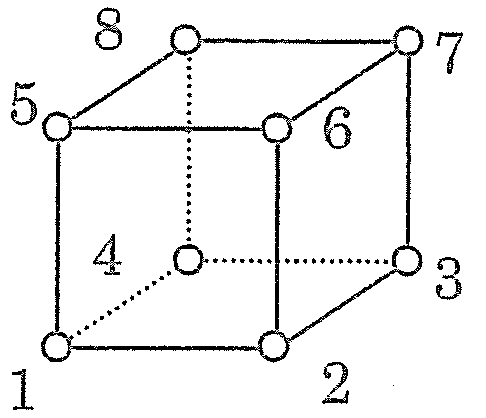
\includegraphics[keepaspectratio]{work/images/hex8.png} 
                     & 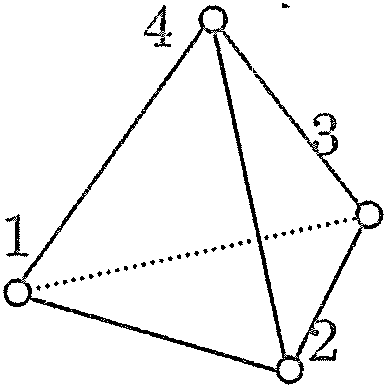
\includegraphics[keepaspectratio]{work/images/tet4.png}  \\
          \hline
          メリット   & 任意の形状で切れる & 見た目が美しい & 無 \\
          \hline
          デメリット & 多少見た目が悪い   & 形状に人間の介入が必要 & 硬い \\
          \hline
          評価       &   〇               & ◎              & × \\
          \hline
    \end{tabular}
  \end{table}
  %
  % TiKZを使った図形の描画 図2でA点を指し示す矢印
  \begin{textblock*}{30pt}(385pt,105pt)
    \begin{tikzpicture}
        \node[rectangle,fill=cud_yellow,text width=0.5cm,text centered,rounded corners,minimum height=0.5cm](s) at (1cm,1cm) { \scriptsize 使用禁止};
    \end{tikzpicture}
  \end{textblock*}
\end{frame}
           % 改めてメッシュについて復習
  \begin{frame}{6面体要素が切れる形状}
  \begin{table}[hbtp]
      \caption{3次元構造解析で使われる主なメッシュ要素(一部)<参考文献\cite{handbook}>}
      \vspace{-5mm}
      \begin{tabular}{|r|c|c|c|} % 表は項目名を右寄せ、データを中寄せ
          \hline
          名称       & 4面体2次要素 & 6面体1次要素 & 4面体1次要素 \\
          \hline
          接点配置   & 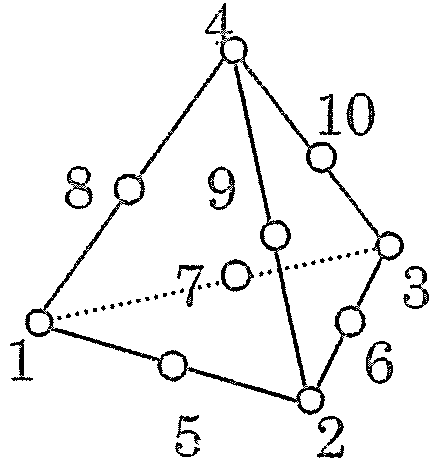
\includegraphics[keepaspectratio]{work/images/tet10.png}
                     & 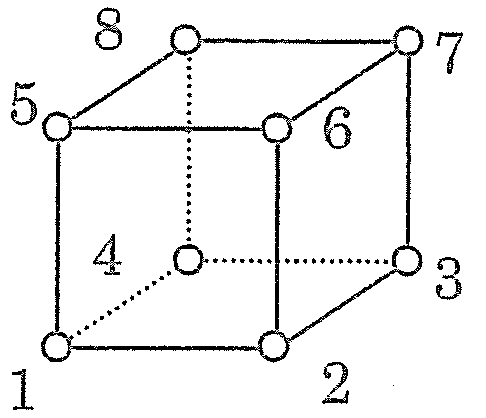
\includegraphics[keepaspectratio]{work/images/hex8.png} 
                     & 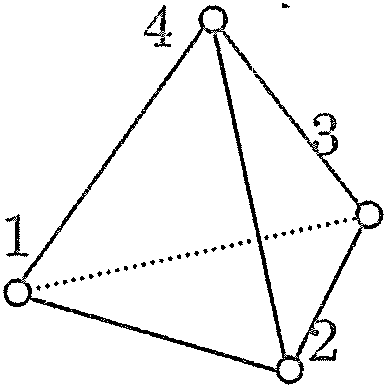
\includegraphics[keepaspectratio]{work/images/tet4.png}  \\
          \hline
          メリット   & 任意の形状で切れる & 見た目が美しい & 無 \\
          \hline
          デメリット & 多少見た目が悪い   & 形状に人間の介入が必要 & 硬い \\
          \hline
          評価       &   〇               & ◎              & × \\
          \hline
    \end{tabular}
  \end{table}
  %
  % TiKZを使った図形の描画 図2でA点を指し示す矢印
  \begin{textblock*}{30pt}(385pt,105pt)
    \begin{tikzpicture}
        \node[rectangle,fill=cud_yellow,text width=0.5cm,text centered,rounded corners,minimum height=0.5cm](s) at (1cm,1cm) { \scriptsize 使用禁止};
    \end{tikzpicture}
  \end{textblock*}
\end{frame}
              % 
  %%%
  \begin{frame}{結果}
 
  半径方向応力については、(最外面、最内面についてはわずかに外れたが) \\
  他は非常によく一致

  周方向応力については、全体的にやや多めに表示されたが、ほぼ一致 
% 図の挿入
\begin{figure}[htbp]
\centering
  \begin{minipage}{0.49\columnwidth}
     \centering
     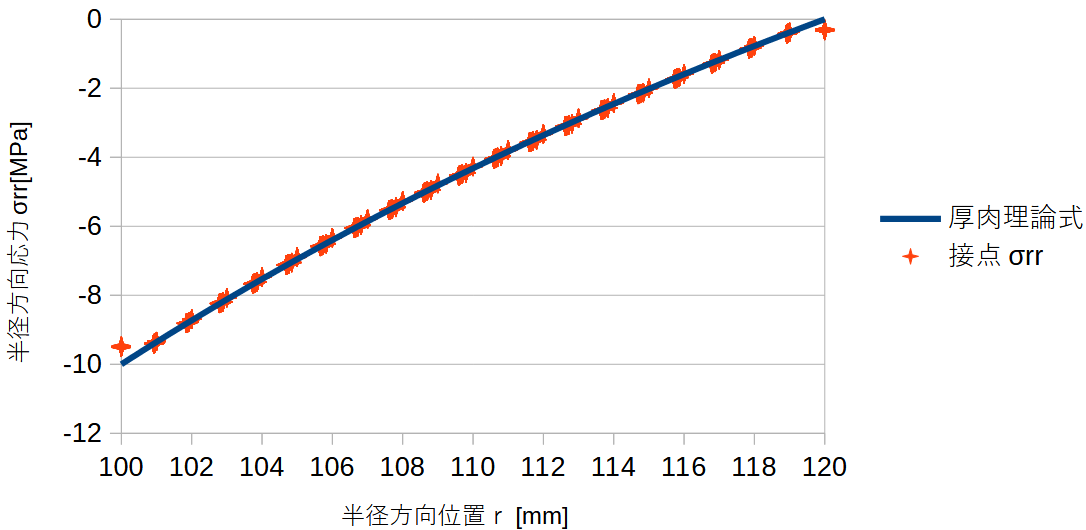
\includegraphics[width=\columnwidth]{work/images/results01.png}
     \caption{半径方向応力σrr}
     \label{fig:hidari}
  \end{minipage}
%
  \begin{minipage}{0.49\columnwidth}
     \centering
     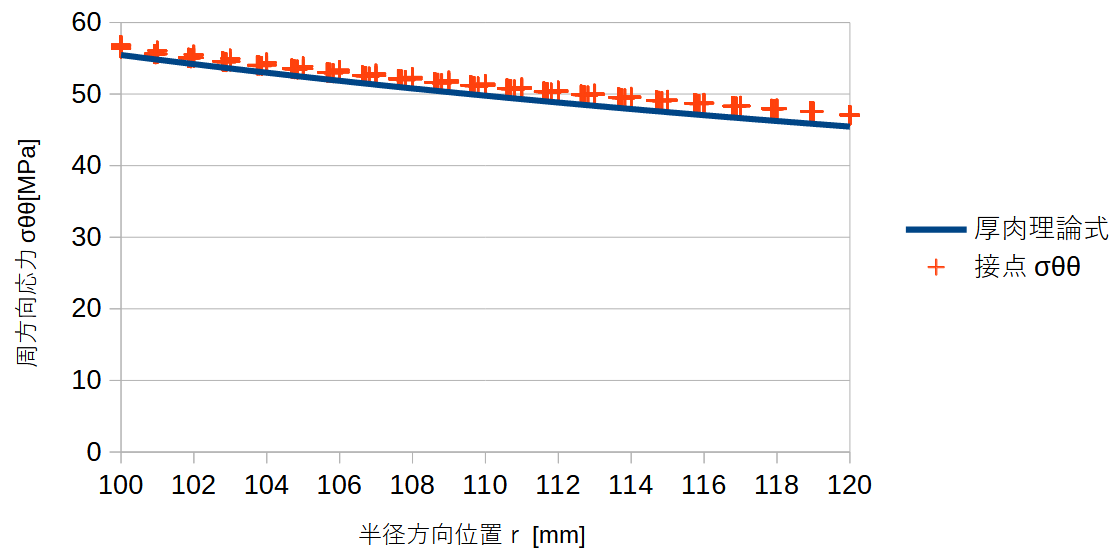
\includegraphics[width=\columnwidth]{work/images/results02.png}
     \caption{周方向応力σθθ}
     \label{fig:migi}
  \end{minipage}
\end{figure}

\end{frame}
         % 結果1
  \begin{frame}{反力のチェックサム(結果)}
 
% PrePoMaxにおいて、反力チェックサムを確認するには、以下設定する \\

 % TiKZを使った図形の描画 図2でA点を指し示す矢印
  \begin{textblock*}{0.95\linewidth}(-10pt,-5pt)
    \begin{figure}[htbp]
      \begin{center}
        \begin{tikzpicture}
	  \node [above right,minimum height=50pt, minimum width=420pt,align=left] at (0pt,0pt) {PrePoMaxにおいて、反力チェックサムを確認するには、以下設定する};
          \node[draw=blue,above right,minimum height=70pt,minimum width=110pt,align=left] at (20pt,-60pt)
		{ \scriptsize{合計された結果を見るには}\\
		  \scriptsize{XX-REACTION-FORCEの}\\
		  \scriptsize{TOATALFORCE-RF1のタグを}\\
		  \scriptsize{確認する}};
          \node[above right,minimum height=170pt,minimum width=260pt,align=left] at (130pt,-160pt) {
	    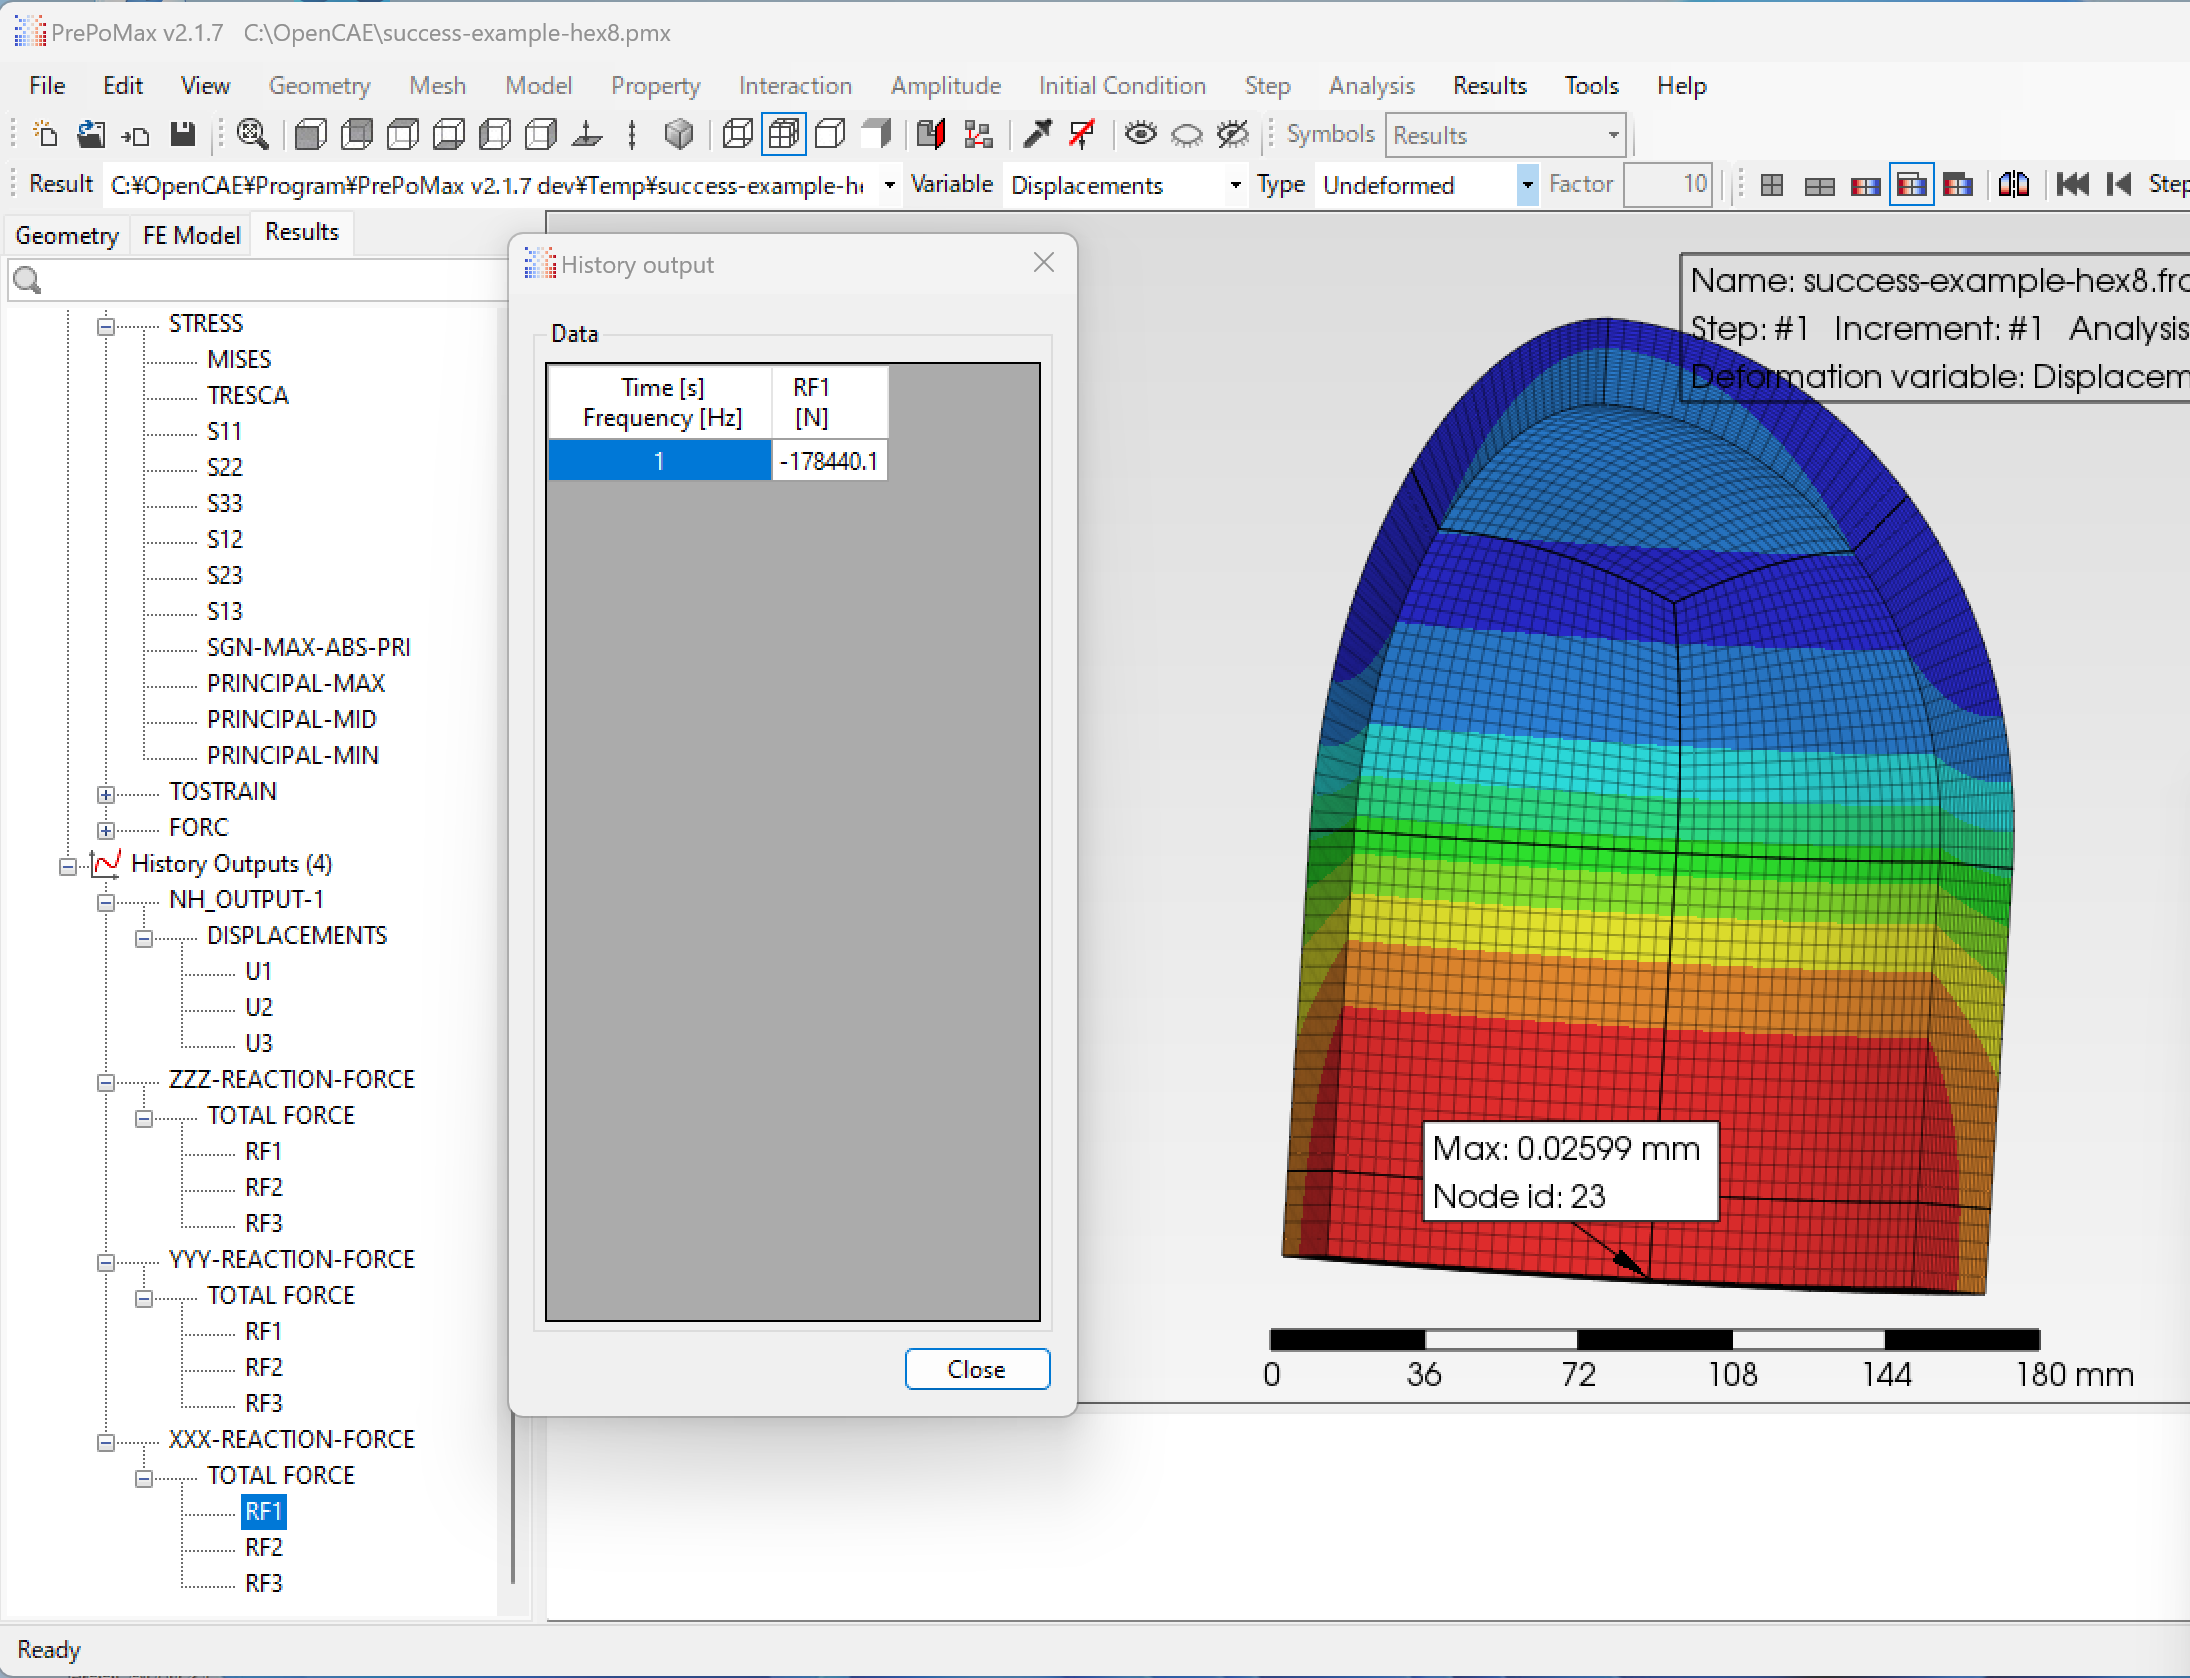
\includegraphics[keepaspectratio,scale=0.265] {work/images/screen02.png}};
          \draw[->, draw=cud_red, line width=1pt] (120pt,-60pt) -- (170pt,-140pt);
          \node[draw=blue,above right,minimum height=70pt,minimum width=100pt,align=left] at (20pt,-160pt)
		{ \scriptsize{この値がX方向から見た}\\
		  \scriptsize{受圧面の投影面積に面圧}\\
		  \scriptsize{をかけたものが}\\
		  \scriptsize{等しいか確認する}\\
		  \scriptsize{今回は誤差0.5\%}};
          \draw[->, draw=cud_red, line width=1pt] (120pt,-120pt) -- (227pt,-35pt);
        \end{tikzpicture}
        \caption{反力チェックサムの確認}
      \end{center}
    \end{figure}
  \end{textblock*}
\end{frame}
         % 結果2
  %%%
  \begin{frame}{本日の流れ}
  \begin{itemize}
      \item[] 目次
      \begin{itemize}[itemsep=1.3ex, leftmargin=1cm]
        \item[1.] {\color{cud_lightgray} 自己紹介}
        \item[2.] {\color{cud_lightgray} 報告者が当時出来ていたこと}
        \item[3.] {\color{cud_lightgray} 本日の例題と以前の勉強会で報告された結果}
        \item[4.] {\color{cud_lightgray} 改めて解いてみた}
        \item[▶5.] \highlight[cud_yellow]{ まとめ }
      \end{itemize}
  \end{itemize}
\end{frame}
           % 
  \begin{frame}{まとめ}
  \begin{itemize}[itemsep=2.5ex, leftmargin=3mm]
      \large
      \item[〇] OpenCAEは、初級の構造解析者が使えるべき機能を \\
                十分に備えている

      \item[〇] 今回の報告では特にメッシュ切を中心にまとめた

      \item[〇] 次回はメッシュ品質についてまとめる予定

  \end{itemize}
\end{frame}
       % まとめ
  %%%
  \begin{frame}{4面体メッシュ切り(成功例)}
 
% 図の挿入
\begin{figure}[htbp]
\begin{center}
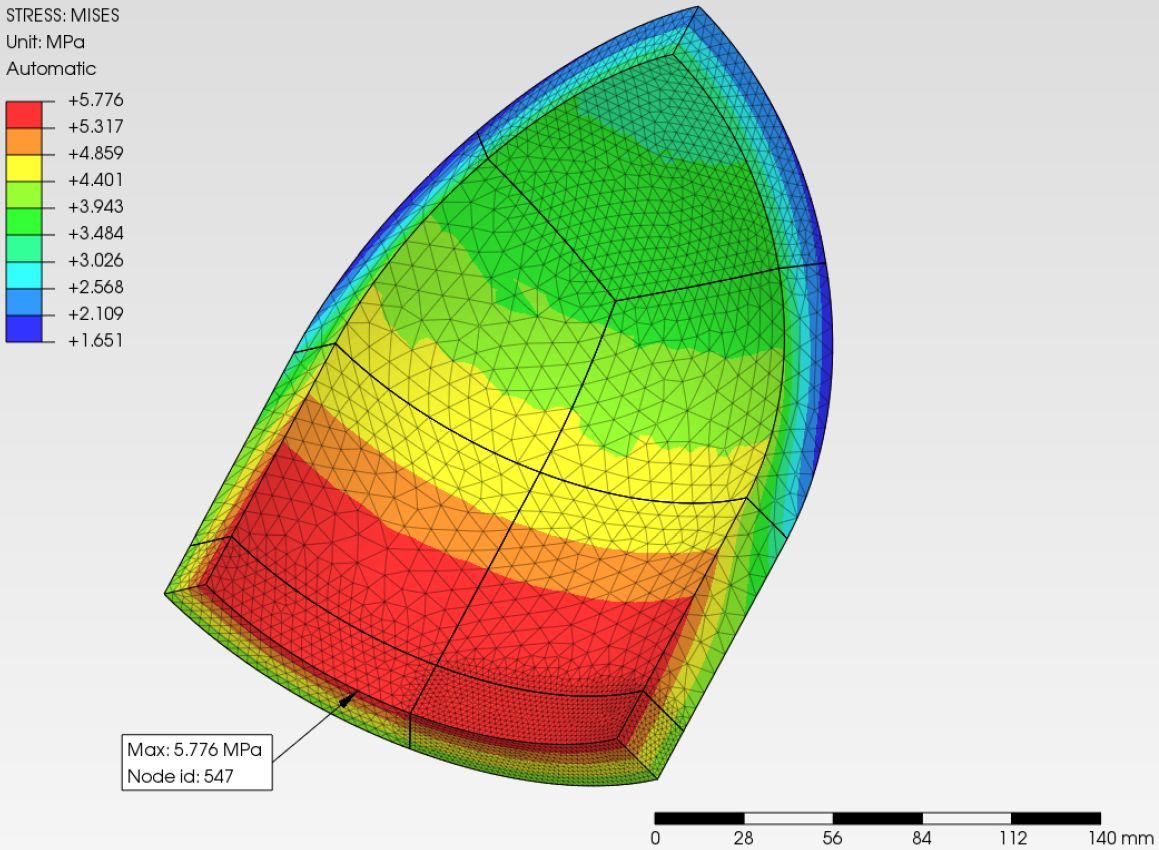
\includegraphics[keepaspectratio,scale=1.0]{work/images/fig01.jpg}
\caption{4面体メッシュ切り(成功例)}
\end{center}
\end{figure}
 
\end{frame}

  \begin{frame}{6面体メッシュ切り(成功例)}
 
% 図の挿入
\begin{figure}[htbp]
\begin{center}
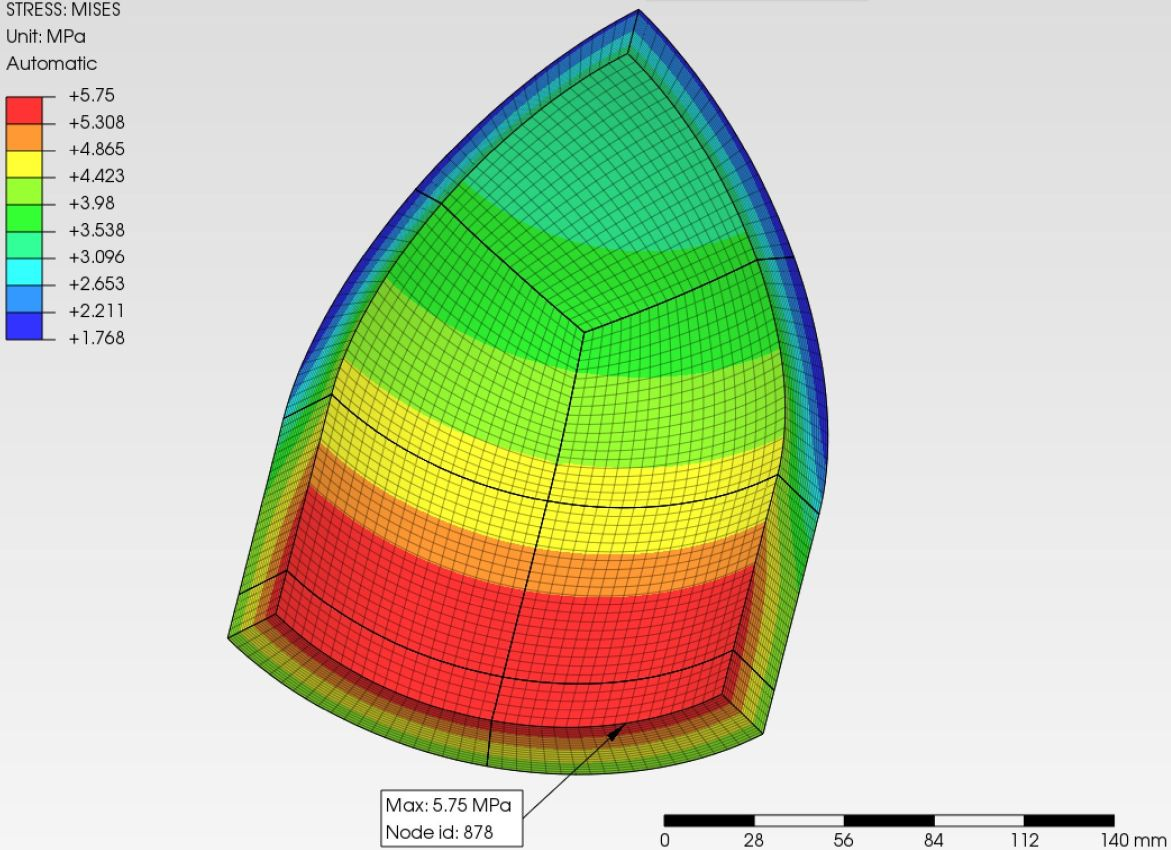
\includegraphics[keepaspectratio,scale=1.0]{work/images/fig02.jpg}
\caption{6面体メッシュ切り(成功例)}
\end{center}
\end{figure}
 
\end{frame}

  \begin{frame}{6面体メッシュ切り(失敗例)}
 
% 図の挿入
\begin{figure}[htbp]
\begin{center}
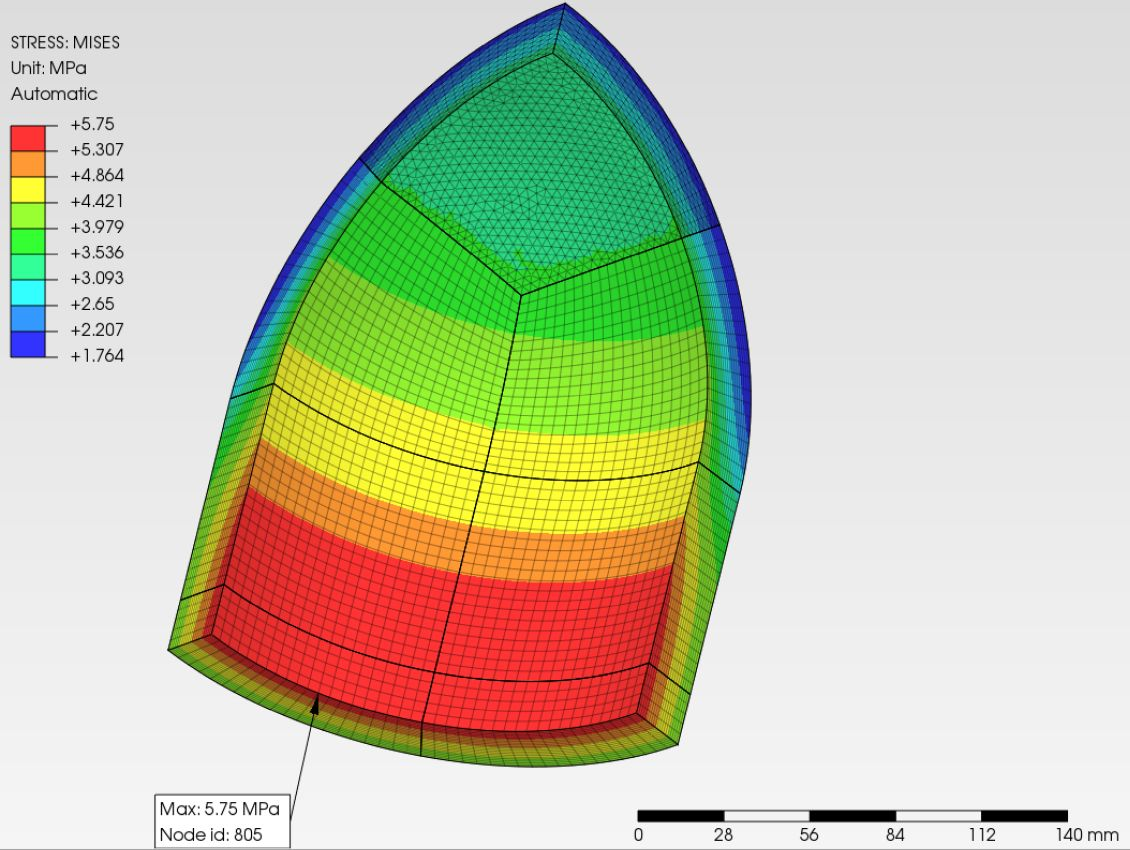
\includegraphics[keepaspectratio,scale=1.0]{work/images/fig03.jpg}
\caption{6面体メッシュ切り(失敗例)}
\end{center}
\end{figure}
\end{frame}

  %%%
  \begin{frame}{参考文献}
  \begin{enumerate}[label=\textbf{[\arabic*]},itemsep=1ex, leftmargin=1mm]
      \item オープンCAE勉強会@関西.“オープンCAE Wanted@関西”.\\
          {\footnotesize \urlstyle{same}
          \url{https://scrapbox.io/opencae-wanted/第76回:圧力容器の応力値を手計算とCAEで比較した}} \\
          (参照 2024-02-23)
     % \item @Sagittarius_Chiron.“PrePoMax使用法解説ー3.0 複合材”.Qiita.\\
      \item @Sagittarius\_Chiron.“PrePoMax使用法解説ー3.0 複合材”.Qiita.\\
          {\footnotesize \urlstyle{same}
          \url{https://qiita.com/Sagittarius_Chiron/items/6a885ea8ee8f35c7a89c}} \\
          (参照 2024-02-23)
  \end{enumerate}
\end{frame}
        % 参考文献
  \begin{frame}[noframenumbering]{}
	ご清聴、ありがとうございました

  % この場合は (150pt, 150pt) の位置に 0.6\linewidth の幅のブロックができる.
  \begin{textblock*}{0.7\linewidth}(100pt,180pt)
    % TiKZを使った図形の描画
    \begin{tikzpicture}
        \node[rectangle,fill=cyan!10,text width=320pt,text centered,rounded corners,minimum height=50pt,align=left]
           { \scriptsize (このスライドのTexソースは \\
             \urlstyle{same}
             \url{https://github.com/ichmy55/opencae-slides/tree/main/src/opencae-kantou-s-025} \\
             にあります。よければご参照ください
           };
    \end{tikzpicture}
  \end{textblock*}
\end{frame}
           % ご清聴、ありがとうございました
  \begin{frame}[noframenumbering]{付録A. ~今回使用した主なソフト~}
  \begin{table}[hbtp]
    \caption{今回使用した主なソフト}
    \vspace{-5mm}
    \begin{tabular}{|c||l|l|l|} \hline % 表は項目名を中央寄せ、データを左寄せ
	    用途          & 名称 & バージョン & URL \\ \hhline{|=:=|=|=|}
      3次元形状作成 & gmsh & 4.13.1 & {\urlstyle{same} \color{cud_orange}
                                   \href{https://gmsh.info}
				   {gmsh.info}}  \\ \hline
      プリ・ポスト  & PrePoMax & 2.1.7 & {\urlstyle{same} \color{cud_orange}
                                   \href{https://prepomax.fs.um.si/}
				   {prepomax.fs.um.si}}  \\ \hline
      ソルバ(PrePoMax同梱) & Calculix & 2.21 & {\urlstyle{same} \color{cud_orange}
                                   \href{https://calculix.de/}
				   {calculix.de}}  \\ \hline
      表計算        & LibreOffice & 24.8.0.3 & {\urlstyle{same} \color{cud_orange}
                                   \href{https://libreoffice.org/}
				   {libreoffice.org}}  \\ \hline
      OS            & Windows & 11Pro(23H2) & {\urlstyle{same} \color{cud_orange}
                                   \href{https://www.microsoft.com/}
				   {microsoft.com}}  \\ \hline
    \end{tabular}
    \\(注:各ソフトはWindows版x86\_64/amd64用を使用しています)
  \end{table}
\end{frame}
      % 付録 ~今回使用したソフト~
  \begin{frame}[noframenumbering]{付録B. ~ソースのありか~}
  \begin{table}[hbtp]
    \caption{ソースのありか}
    \vspace{-7mm}
    \begin{tabular}{|r||l|l|} \hline % 表は項目名を右寄せ、データを左寄せ
      項目                & 置き場 & URL \\ \hhline{|=:=|=|}
        レジストリ & \multirow{3}{*}{Github} & {\urlstyle{same} \color{cud_orange}
                        \href{https://github.com/ichmy55/opencae-slides}
                         {github.com/ichmy55/opencae-slides}} \\  \cline{1-1} \cline{3-3}
        \multirow{2}{*}{配布物} & & \color{cud_orange}
                         github.com/ichmy55/opencae-slides/releases/ \\
                   & & {\urlstyle{same} \color{cud_orange}
                           \href{https://github.com/ichmy55/opencae-slides/releases/download/v0.2.18/Handout.zip}
                         {releases/download/v0.2.18/Handout.zip}} \\ \hline
        図面       &  Onshape &  {\footnotesize
	                           {\urlstyle{same} \color{cud_orange}
                                     \href{https://cad.onshape.com/documents/8308453c2a5cbbceb286aa1a/w/1773f76374703247baf0d72a/e/bbd26f6d00f1e7f89db44d66}
					{予定地}}(今回報告では未対応)} \\ \hline
        スライド.pdf  & Docswell & {\urlstyle{same} \color{cud_orange}
                                   \href{https://www.docswell.com/user/ichmy55}
                                   {www.docswell.com/user/ichmy55}} \\ \hline
    \end{tabular}
  \end{table}
\end{frame}
      % 付録 ~配布するデータファイル~
  \begin{frame}[noframenumbering]{付録C. ~配布するデータファイル~}
  前ページで示した配布物の中身は以下のとおり
   \begin{table}[hbtp]
    \caption{Handout.zipの中身}
    \vspace{-2mm}
   {\scriptsize
      \begin{tabular}{|c||l|l|l|} \hline % 表は項目名を中央寄せ、データを左寄せ
        ディレクトリ & ファイル種類 & ファイル名 & 概要 \\ \hhline{|=:=|=|=|}
	\multirow{2}{*}{01-gmsh-script} & gmsh入力  & failure-example.geo & メッシュ切失敗形状  \\ \cline{3-4}
				        & スクリプト& successful-example.geo & メッシュ切成功形状  \\ \hline
        \multirow{4}{*}{02-gmsh-shape}  & gmsh形状出力  & failure-example.brep & メッシュ切失敗形状  \\ \cline{3-4}
				        & B-rep形式 & successful-example.brep & メッシュ切成功形状  \\ \cline{2-4}
                                        & gmsh形状出力  & failure-example.step & メッシュ切失敗形状  \\ \cline{3-4}
                                        & step形式  & successful-example.step & メッシュ切成功形状  \\ \hline
        03-prepomax-savefile            & prepomaxセーブ  & success-example-hex8.pmx &   \\ \hline
        04-calculix-input               & calculix入力 & success-example-hex8.inp &   \\ \hline
   \multirow{2}{*}{05-caluculix-output} & \multirow{2}{*}{ocalculix出力}  & success-example-hex8.frd & 全接点応力出力  \\ \cline{3-4}
				        & & success-example-hex8.dat & 特定接点変位出力  \\ \hline
        06-libreoffice                  & 表計算 & successful-example-hex8.ods &   \\ \hline
      \end{tabular}
    }
  \end{table}
\end{frame}
      % 付録 ~ソースのありか~
\end{document}
